\chapter{Experiments} % Main chapter title

\label{chapter4} % Change X to a consecutive number; for referencing this chapter elsewhere, use \ref{ChapterX}

\lhead{Chapter 4. \emph{Experiments}} 
\label{chapter::experiments}

In this section we report evaluations for our proposed approach. We compare our
tracking ensemble method and other state-of-the-art trackers using complete
50 sequences tracking benchmark \cite{Wu2013B}. We also present qualitative and
quantitative analysis of our ensemble tracker, such as
individual performance of trackers and effect of the tracker pool.

\section{Implementation details}
We implemented our online ensemble approach in MATLAB. CL clustering method is
implemented in C++ and ported as \textit{mex} function. Object model corresponds
to a standard RBF SVM, implemented in LIBSVM library \cite{libsvm}. To extract
HOG features, we made use of Piotr Toolbox for Matlab \cite{PMT} using default parameters. All experiments were performed on a PC with an Intel Xeon CPU and 16 GB of RAM.

\section{Evaluation Metrics}
The trackers were put into test using two evaluation metrics commonly employed in
the literature. The first is \textit{distance precision} (DP), which is the number
of frames where the estimated center location is within a certain distance
threshold $d$ from the \gls{gt} center location. The second metric is
\textit{overlap precision} (OP), defined as the number of frames where the
overlap between the estimated and ground truth bounding box exceeds
a threshold $b$. On each sequence, these two measures are calculated using
equations \ref{eq::precision} and \ref{eq::overlap}. Estimated center location
and \gls{gt} are denoted as $\mathbf{p}_f$ and $\mathbf{\hat{p}}_f$
respectively, where $f$ is the frame number. Futhermore, $B_f$ and $\hat{B}_f$
denote the estimated and ground truth bounding boxes of the object. $N$ is the
number of frames in the sequence.

\begin{subequations}
\begin{equation}
	\mathrm{DP}(d) = \frac{1}{N}|\{f:||\mathbf{\hat{p}}_f - \mathbf{p}_f|| \leq d\}|,\:d\geq 0
\label{eq::precision}
\end{equation}

\begin{equation}
	\mathrm{OP}(b) = \frac{1}{N}\left | \left \{ f: \frac{|\hat{B}_f \bigcap B_f|}
										{|\hat{B}_f \bigcup  B_f|}
	 \geq b \right \} \right |,\:0 \leq b\leq 1
\label{eq::overlap}
\end{equation}
\end{subequations}

In the recent literature, there has not been much agreement on which
performance measure to use for comparing visual trackers. DP focuses only
on estimated center location, which is beneficial for trackers that do not
estimate scale of the object. Instead, OP also takes estimated scale into
account and penalizes if the scale of the target is estimated incorrectly.

Recently, the authors of Online Object Tracking Benchmark (OOTB) \cite{Wu2013B} suggest the usage
of precision and success plots. These curves show distance and \gls{overlap} precision metrics over a range of
thresholds. For instance, in precision plot, a higher precision at low
thresholds means the tracker is more accurate, while a lost target will not
achieve perfect precision on a large threshold range. In both types of plots,
a \textit{ranking score} is computed to line up trackers overall performance.
In precision plot, the DP value of 20 pixels is used as ranking score. In contrast to precision, in success plots, trackers are ranked using area under
the curve (AUC), which relates to the average overlap across all frames. 

To validate the performance of our proposed approach, we follow the one-pass
evaluation methodology (OPE) proposed in \cite{Wu2013B}. OPE evaluates trackers
performance running them throughout a test sequence with initialization from
the \gls{gt} position in the first frame. We summarize results using the precision and
success plots in the complete dataset.

\begin{table}[h!]
\caption[Selected tracking algorithms for ensemble method.]{\small Selected tracking algorithms for ensemble method. \textbf{Code Column}: 
M: Matlab, MC: Mixture of Matlab and C/C++, other: DLL files.}
\resizebox{\linewidth}{!}{%
\begin{tabular}{llll}
\toprule
 \textbf{Method}&  \textbf{Type}& \textbf{Code}& \\ \midrule
 Template matching - TM \cite{Collins2005a}& Template-based& other&  \\
 Mean Shift - MS \cite{Collins2005a}& Density-based& other&  \\
 Variance Ratio - VR \cite{Collins2005a}& Density-based& other&  \\
 Peak Difference - PD \cite{Collins2005a}& Point-based& other&  \\
 Ratio Shift - RS \cite{Collins2005a}& Point-based& other&  \\ 
 Adaptive Structural Local Sparse Appearance \\ Model - ASLA \cite{Jia2012}& Sparse representation&  MC& 
 \\  Compressive Tracker - CT \cite{Zhang2012}& Sparse representation& MC&  \\
 Minimum Experts Entropy Minimization - MEEM \cite{zhang2014meem}& tracking by detection& MC&  \\ 
 Self-paced learning for long-term tracking - SPLTT \cite{Supancic2013}& tracking by detection& MC& \\ 
 Kernelized Correlation Filters - KCF \cite{Henriques2014}& Template-based& M&  \\ 
 Dual Correlation Filters - DCF \cite{Henriques2014}& Template-based& M&  \\  
 Spatio-temporal Context Tracker - SCT \cite{Zhang2013}& Template-based& M&  \\
 Circulant Structure Kernel - CSK, sKCF \cite{Henriques2014}& Template-based& M&  \\
 Robust CSK tracker - RCSK \cite{Danelljan2014}& Template-based& M&\\  
 Minimum Output Sum of Squared Error - MOSSE \cite{Bolme2010}& Template-based& M&  \\ 
\bottomrule
\end{tabular}}
\label{table:trackers}
\end{table}

\section{Dataset}
In order to evaluate the performance of our proposed ensemble tracking,
we adopt the OOTB from \cite{Wu2013B}.
This is an extensive benchmarking dataset that includes 50 sequences
annotated with 11 attributes.
The dataset includes challenging scenarios such as motion blur,
illumination changes, scale variation, occlusions,
in-plane and out-of-plane rotations, object deformation,
background clutter and low resolution. The selection criteria of this dataset
are listed below. 
\begin{itemize}
\item \textbf{Standarized sequences: }For better comparison, OOTB videos are
widely used as benchmark sequences in recent literature, allowing us to make a
fair comparison to state-of-the-art algorithms. Also, all of the sequences were
selected for generic single-object tracking purposes.
\item \textbf{Manual annotations available: }OOTB provides \gls{gt} annotations for
each sequence. This avoids a costly labeling process.
\item \textbf{Image frames: } Each sequence corresponds to a set of image frames. This
format allows to evaluate global processing time of the ensemble approach.
\item \textbf{Attributes classification: } Each sequence provides an annotation with 11
attributes, which explain the challenging scenarios encountered. This
allows us to make attribute-based comparisons, which can show strengths and weaknesses of different trackers.

\end{itemize}

\section{Tracker pool}

%All trackers were modified in order to store their results and save
%their states on each frame.
Table \ref{table:trackers} shows the list of the
selected tracking algorithms that will be included in the pool for our
experiments. The selection criteria for the trackers are
listed below.
\begin{itemize}
\item \textbf{Source code: } We integrate into our pool, tracking algorithms
whose original source code is publicly available. Executable files were not
selected.
\item \textbf{Store current state: } On each frame, a tracker must be able to
store current state and give current result. This allow the ensemble to
perform spatial clustering and compute appearance score for each tracker.
\item \textbf{Trackers bounding box result: } Each tracker estimate must give
current target location and scale overall frames. Also, the current result
must be able to be transformed into a generic format, in order to perform ensemble.
\item \textbf{Reinitialization available: } A tracker is able to reset its
state using final ensemble tracking result.
\end{itemize}

\section{Benchmarking results}

We report the performance of our ensemble tracking algorithm on the 50
benchmarking sequences in
Figure \ref{fig:results}.
The plots compare our approach with each individual tracker
in Table \ref{table:trackers} and state-of-the-art trackers: Struck tracker
\cite{Hare2011}, Sparse Collaborative Model (SCM) \cite{Zhong2012}, TLD tracker
\cite{Kalal2011}. Our online ensemble tracking algorithm is denoted \textit{OET}.

\begin{figure}[h!]
\centering
\subfloat{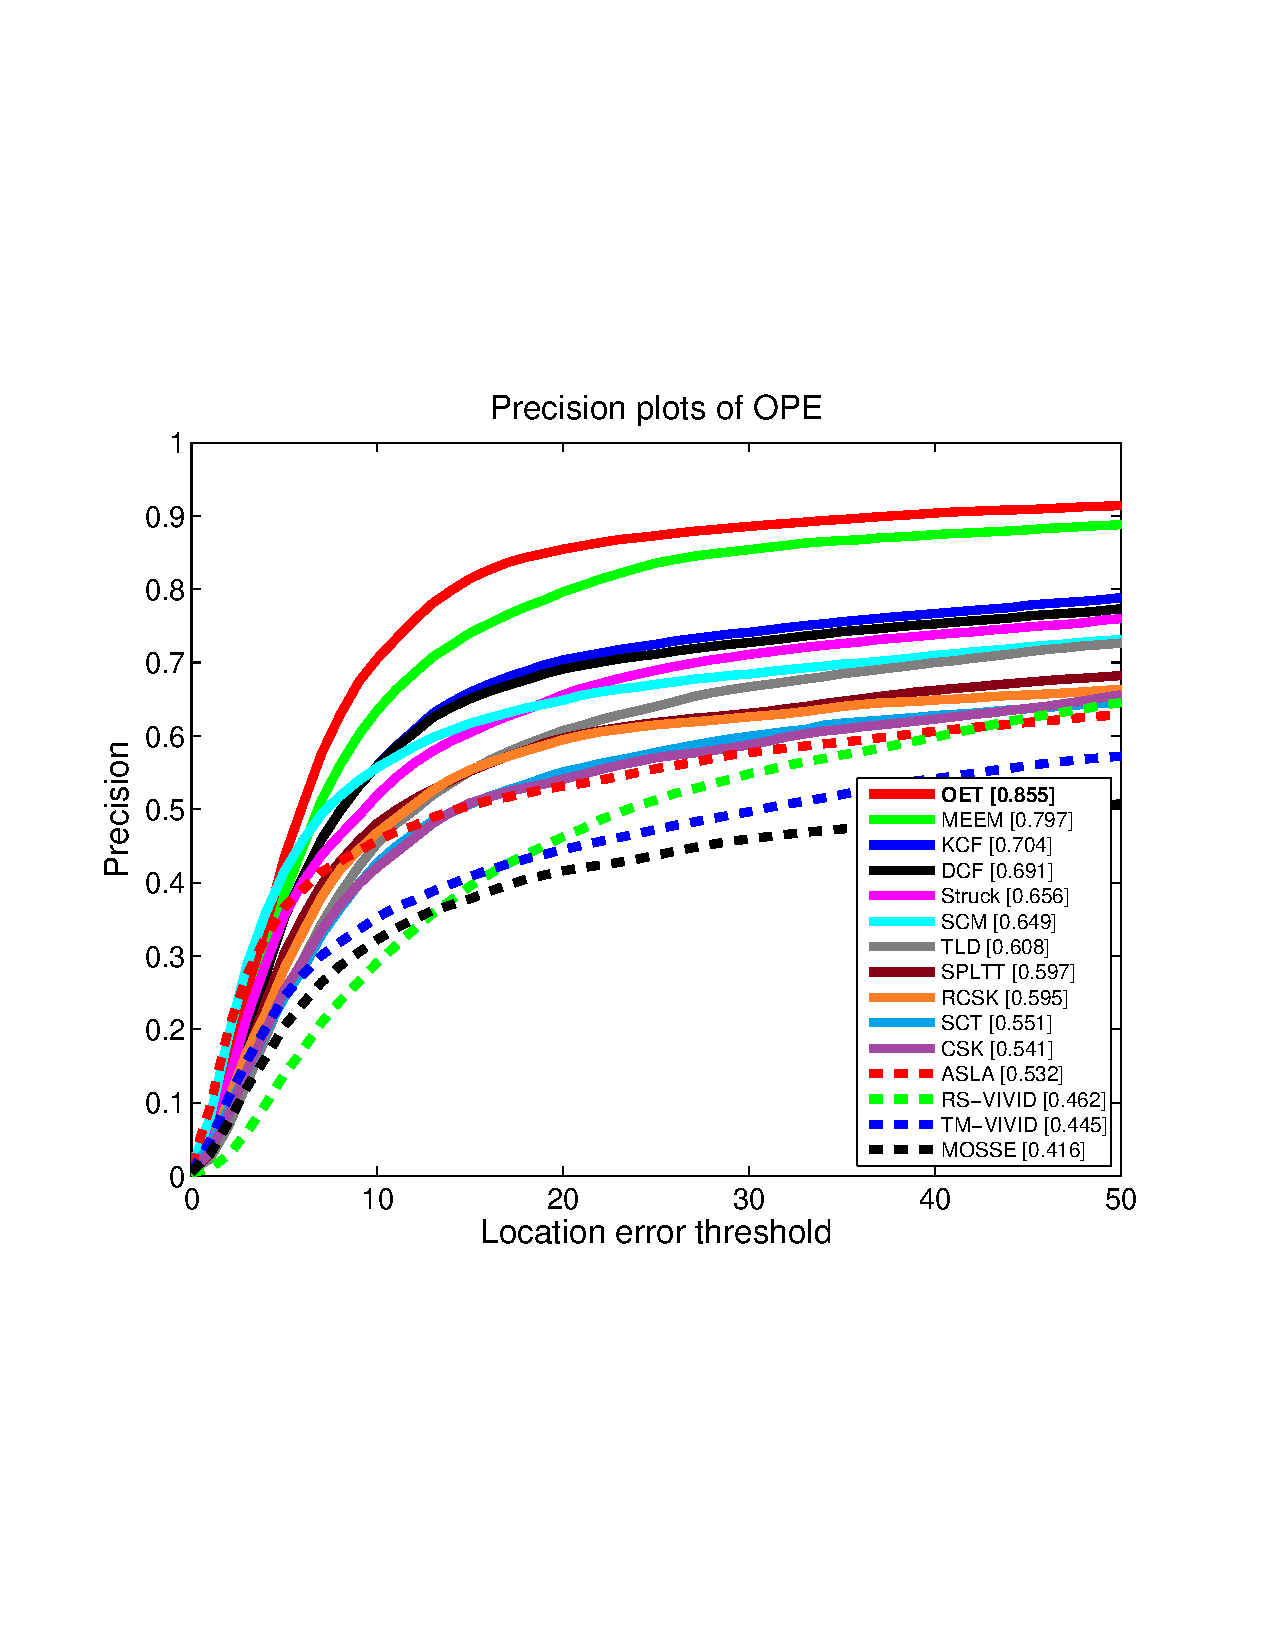
\includegraphics[width=0.5\linewidth, trim= 1cm 6.7cm 2cm 6cm, clip=true]{Figures/Results/quality_plot_error_OPE_threshold}
\label{fig:precision_plot}
}
\subfloat{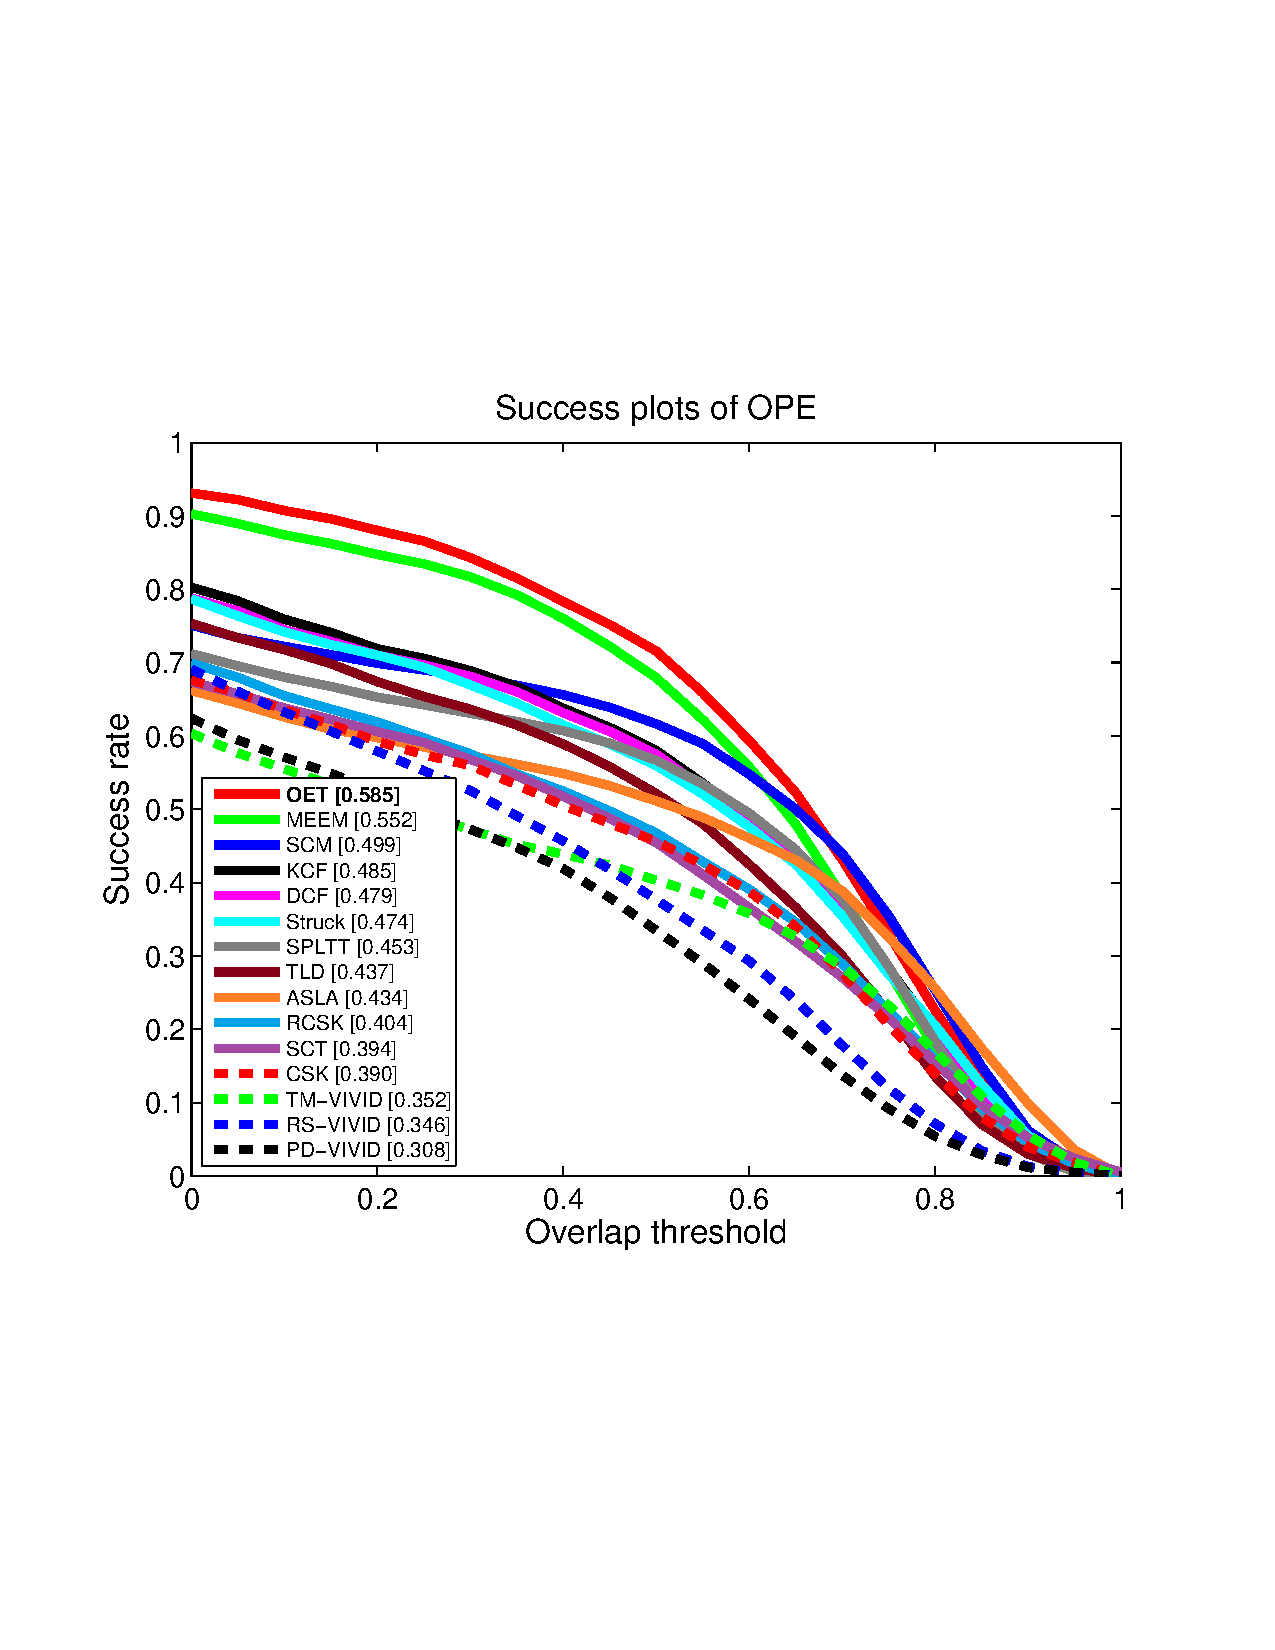
\includegraphics[width=0.5\linewidth, trim= 1cm 6.7cm 2cm 6cm, clip=true]{Figures/Results/quality_plot_overlap_OPE_AUC}
\label{fig:success_plot}
}
\caption[Precision and success plots for all 50 sequences]{\small  Precision and success plots for all 50 sequences. Precision and success
		ratios are measured by center location error and overlap ratio,
		respectively. Trackers are ranked using scores of 20 pixels for
		precision and AUC for success.}
\label{fig:results}
\end{figure}

We note that our tracking ensemble improves performance over current
state-of-the-art tracking algorithms in the benchmark.
From Figure \ref{fig:results}, our method outperforms each individual tracking
score, in both precision and success.
When inspecting individial sequences, we note that 
our method handles camera rotation sequences better, such as \textit{singer1, 
singer2, fish, car4}, unlike the competing
MEEM tracker. Also, our ensemble method can overcome complete object occlusion. In
sequences where this situation happens \textit{jogging, david3}, KCF trackers
fails tracking the object. 

%Establishing a general comparison, performance of MEEM is comparable to ours.
%However,  MEEM tracker fails handling camera rotation as in  sequences. Also, KCF tracker bring good tracking results.
%But, KCF usually fails handling complete objects occlusion. It is good to note,
%as in \cite{Bailer2014}, in our system, scale is not determined. We are
%dependent of each separated tracker scale, and some trackers do not consider
%scale correction. Some of them apply initialization scale over all sequence.
%However, our method outperforms each individual tracker and state-of-the-art
%trackers in success plot, where scale is considered.


\section{Analysis of the tracking ensemble}
\begin{figure}[b!]
\centering
	\figuresr{subway/041}
	\figuresr{subway/042}
	\figuresr{subway/043}
	\figuresr{subway/044}
	\figuresr{subway/045} \\
	\hspace{0.05cm}
	\figuresr{soccer/090}
	\figuresr{soccer/110}
	\figuresr{soccer/131}
	\figuresr{soccer/140}
	\figuresr{soccer/150}
\vspace{-2mm}
\caption[Qualitative results for object tracking applying both inliers selection
	methods
	in two sequences.]{\small Qualitative results for object tracking applying both inliers selection methods in two sequences. \textbf{Green} bounding box corresponds to
	appearance score selection. \textbf{Blue} box to cluster size. In
	\textit{subway} when occlusion happens, many trackers are lost, creating a
	big cluster. In cases of background clutter \textit{soccer}, appearance
	selection loses target in some frames.}
\label{fig::clustvsapp}
\end{figure}


In this subsection, we focus on the relevance of the number of trackers in the pool.
We vary the size of the tracker pool in order to evaluate its effect on the
performance of the ensemble.
When selecting small tracker pools, we first chose the best 5 trackers
from Fig.~\ref{fig:success_plot}. We then augment the pool with the next 5 trackers to
form a pool of size 10. Finally we add the worst 5 trackers for a pool of size 15.
%Finally, we add 5 last trackers.
We also study the effect of the inlier selection criteria of Section
\ref{sec:inliers}
(appearance score and cluster size).

\begin{table}[h!]
\centering
\caption{\small Average AUC and precision for inliers selection methods.}
\resizebox{0.9\linewidth}{!}{%
\begin{tabular}{llll}
\hline
\textbf{Method}     & \textbf{\# trackers} & \textbf{Success(AUC)} & \textbf{Precision(20px)} \\
\hline
           & 5                  & 0.585        & 0.855           \\
\textbf{Appearance score} & 10                 & 0.569        & 0.811           \\
           & 15                 & 0.560         & 0.804           \\
\hline           
           & 5                  & 0.528        & 0.765           \\
\textbf{Cluster size}    & 10                 & 0.493        & 0.715           \\
           & 15                 & 0.480         & 0.678           \\
\hline
\end{tabular}}
\label{table:trackers_number}
\end{table}

The results are summarized in Table \ref{table:trackers_number} for all 50
sequences in the benchmark.
We report AUC ranking score for success, 
and 20-pixel threshold for precision.
%
%Table \ref{table:trackers_number} summarizes quantitative evaluation results for
%all 50 sequences.
%
Our algorithm generally outperforms other methods using
appearance score selection criteria. In case of cluster size selection,
this method usually fails handling occlusions. In some sequences, many trackers
lose object target and keep steady when occlusion happens, creating a big
cluster which has the biggest number of members (Figure \ref{fig::clustvsapp}).
However, this method is smoother and handles better fast motion and background
clutter sequences.

\begin{figure*}
\centering
\subfloat[bolt sequence.]{
	\figuresall{bolt/015}
	\figuresall{bolt/196}
	\figuresall{bolt/236}
	\figuresall{bolt/316}
	\figuresall{bolt/346}	
}

\vspace{-0.3cm}

\subfloat[jogging-2 sequence.]{
	\figuresall{jogging-2/033}
	\figuresall{jogging-2/071}
	\figuresall{jogging-2/104}
	\figuresall{jogging-2/258}
	\figuresall{jogging-2/305}	
}

\vspace{-0.6cm}

\subfloat[singer-1 sequence.]{
	\figuresall{singer-1/048}
	\figuresall{singer-1/131}
	\figuresall{singer-1/179}
	\figuresall{singer-1/242}
	\figuresall{singer-1/306}	
}

\vspace{-0.45cm}

\subfloat[football sequence.]{
	\figuresall{football/005}
	\figuresall{football/086}
	\figuresall{football/135}
	\figuresall{football/325}
	\figuresall{football/353}	
}

\vspace{-0.55cm}

\subfloat[singer-2 sequence.]{
	\figuresall{singer-2/029}
	\figuresall{singer-2/069}
	\figuresall{singer-2/155}
	\figuresall{singer-2/211}
	\figuresall{singer-2/309}	
}

\vspace{-0.65cm}

\subfloat[skating1 sequence.]{
	\figuresall{skating1/058}
	\figuresall{skating1/093}
	\figuresall{skating1/237}
	\figuresall{skating1/295}
	\figuresall{skating1/329}	
}

\vspace{-0.25cm}

\subfloat[david3 sequence.]{
	\figuresall{david3/072}
	\figuresall{david3/092}
	\figuresall{david3/197}
	\figuresall{david3/218}
	\figuresall{david3/242}	
}\\
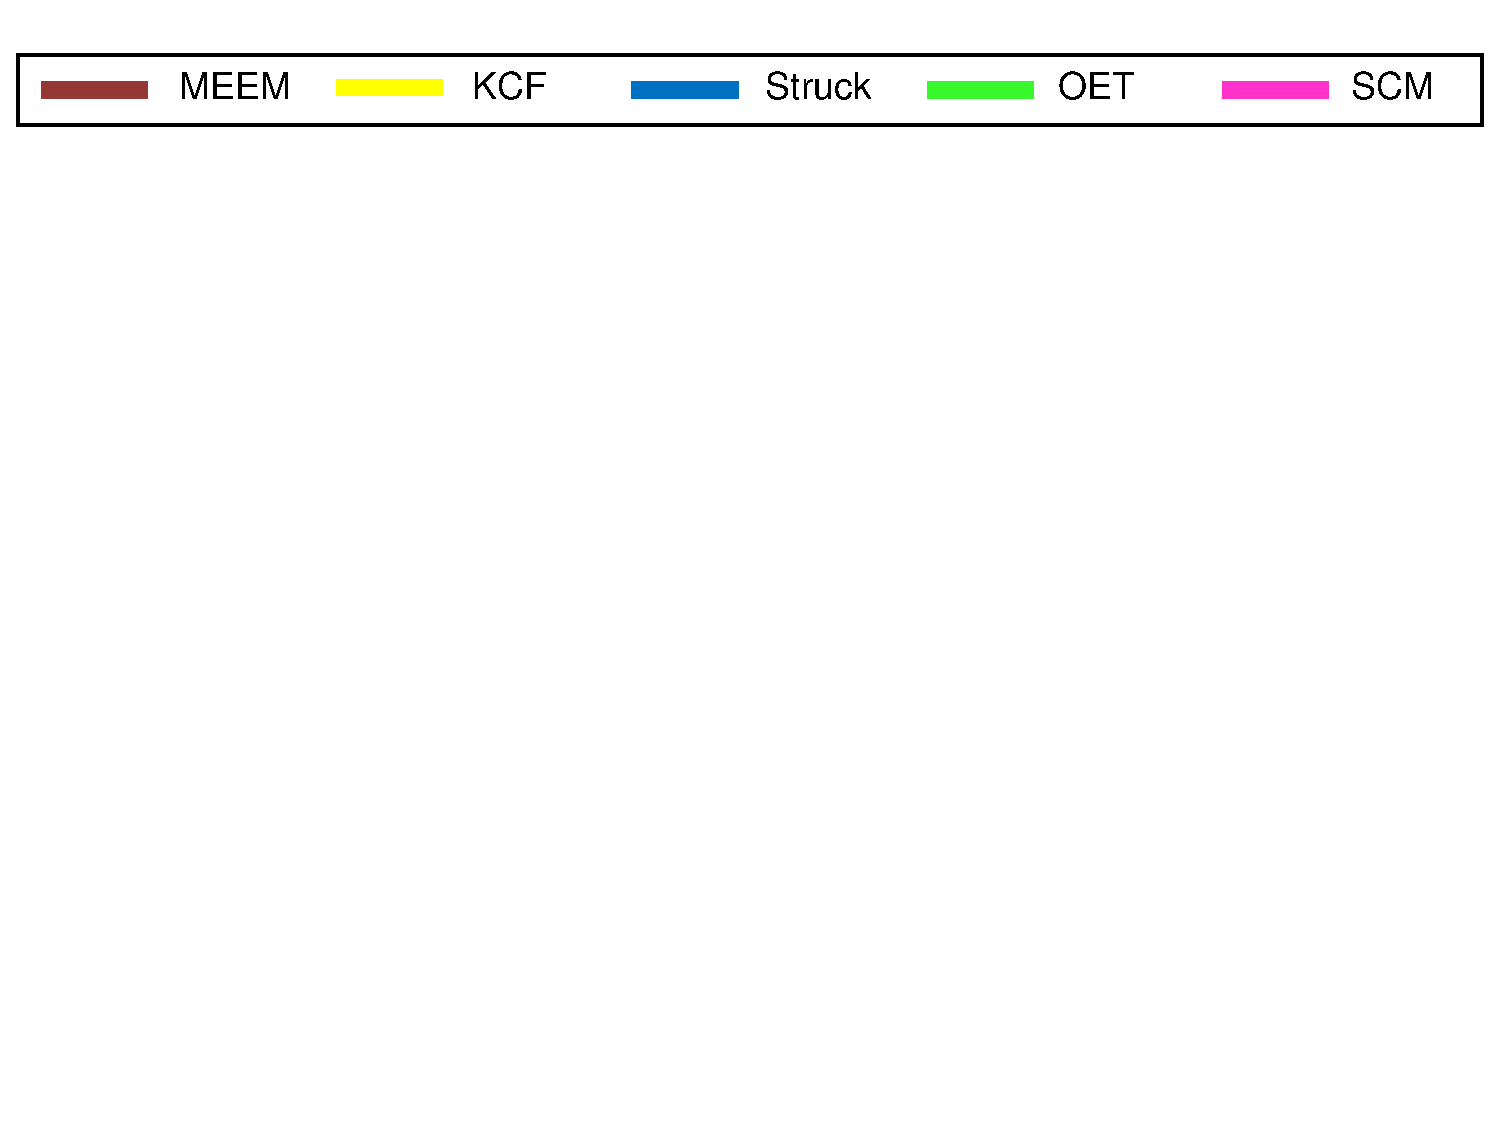
\includegraphics[width=0.8\linewidth, trim= 0cm 16cm 0cm 0cm, clip=true]{Figures/results_all/legend}
\vspace{-0.25cm}
\caption{\small Screenshots of tracking results.}
\end{figure*}

We also note that adding trackers with lower performance hurts the ensemble.
However, the drop in performance when adding
weaker trackers, is less than 5\% ($\sim$1500 frames out of 29519) in success and 10
\% in
precision ($\sim$3000 frames). For instance, when performing inlier selection using
the
appearance score criteria, a spurious tracker may focus on a region with
very similar apperance to the object, \eg background clutter, which can
make tracking fail.
This is very common in the \textit{soccer} and \textit{shaking}
sequences.

In terms of running time, the average time cost for our ensemble
method is $0.062$ s/frame for 5
trackers, $0.122$ s/frame for 10 trackers, and $0.198$ s/frame for 15 trackers.
These timings do not include the processing time of each tracker.
%didn't consider each tracker processing time and model update for timing.

\begin{figure}[h!]
\centering
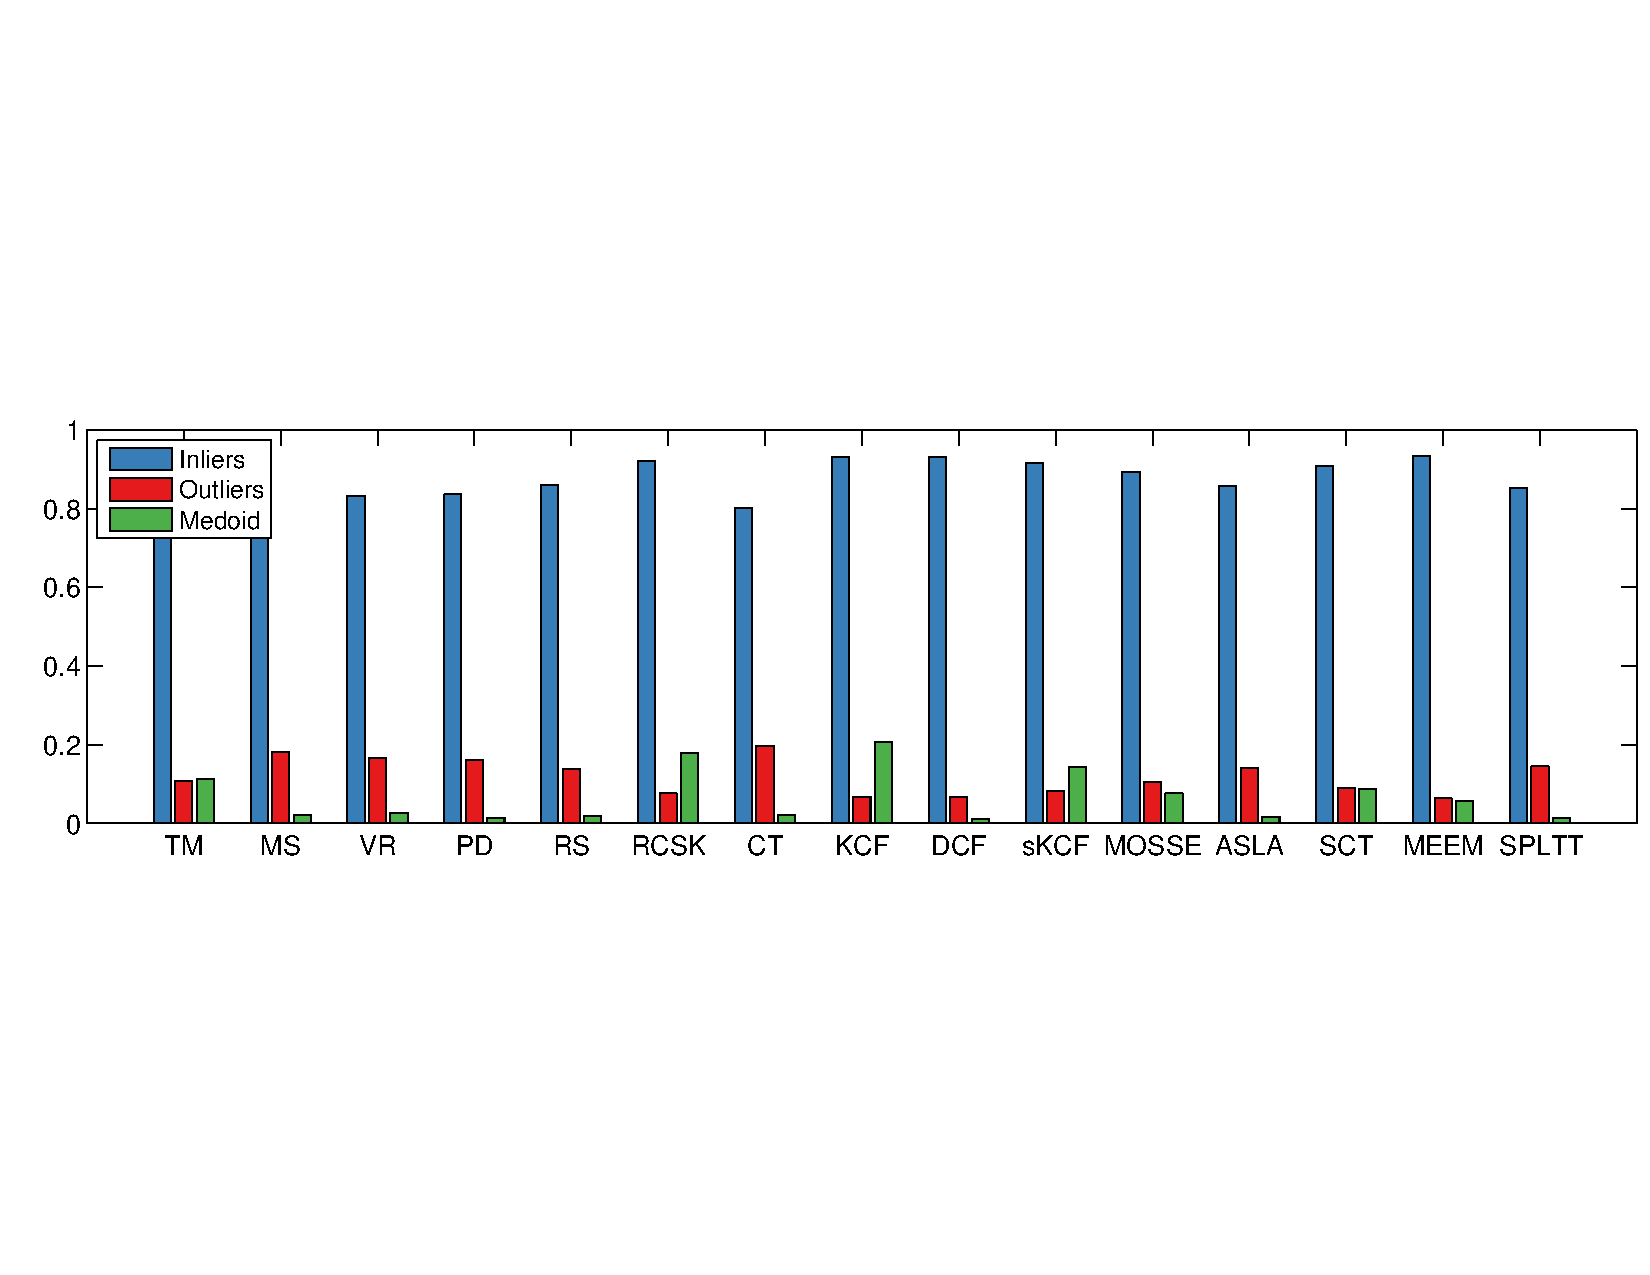
\includegraphics[width=1.0\linewidth, trim= 0.7cm 6.8cm 0.0cm 7.2cm, clip=true]{Figures/test.pdf}
\caption{\small Statistics for each tracker in the ensemble over all frames. }
\label{fig:stats}
\end{figure}

On the other hand, we present statistics about how often trackers in the pool
are selected as outlier, inliner, and medoid.
In figure
\ref{fig:stats}, for each tracker, there are 3 bars: percentage of frames that a
tracker was in best cluster(inlier - blue bar); percentage of frames where a
tracker was considered outlier (red bar); finally, percentage of frames that a
tracker was selected as medoid bounding box (green bar). Based on this result,
trackers whose individual performance is very high, have low percentage of being
considered outliers (KCF, MEEM, RCSK). MEEM individual performance is very high.
However, it does not have the highest frame percentage of being selected as
central bounding box, in comparison with KCF or RCSK. Also, trackers that were
considered spurious in previous experiments, have high rate in outliers bar
(MS, VR, PD, RS). 

\section{Experiments with sequence attributes}

\begin{figure}[h!]
\centering
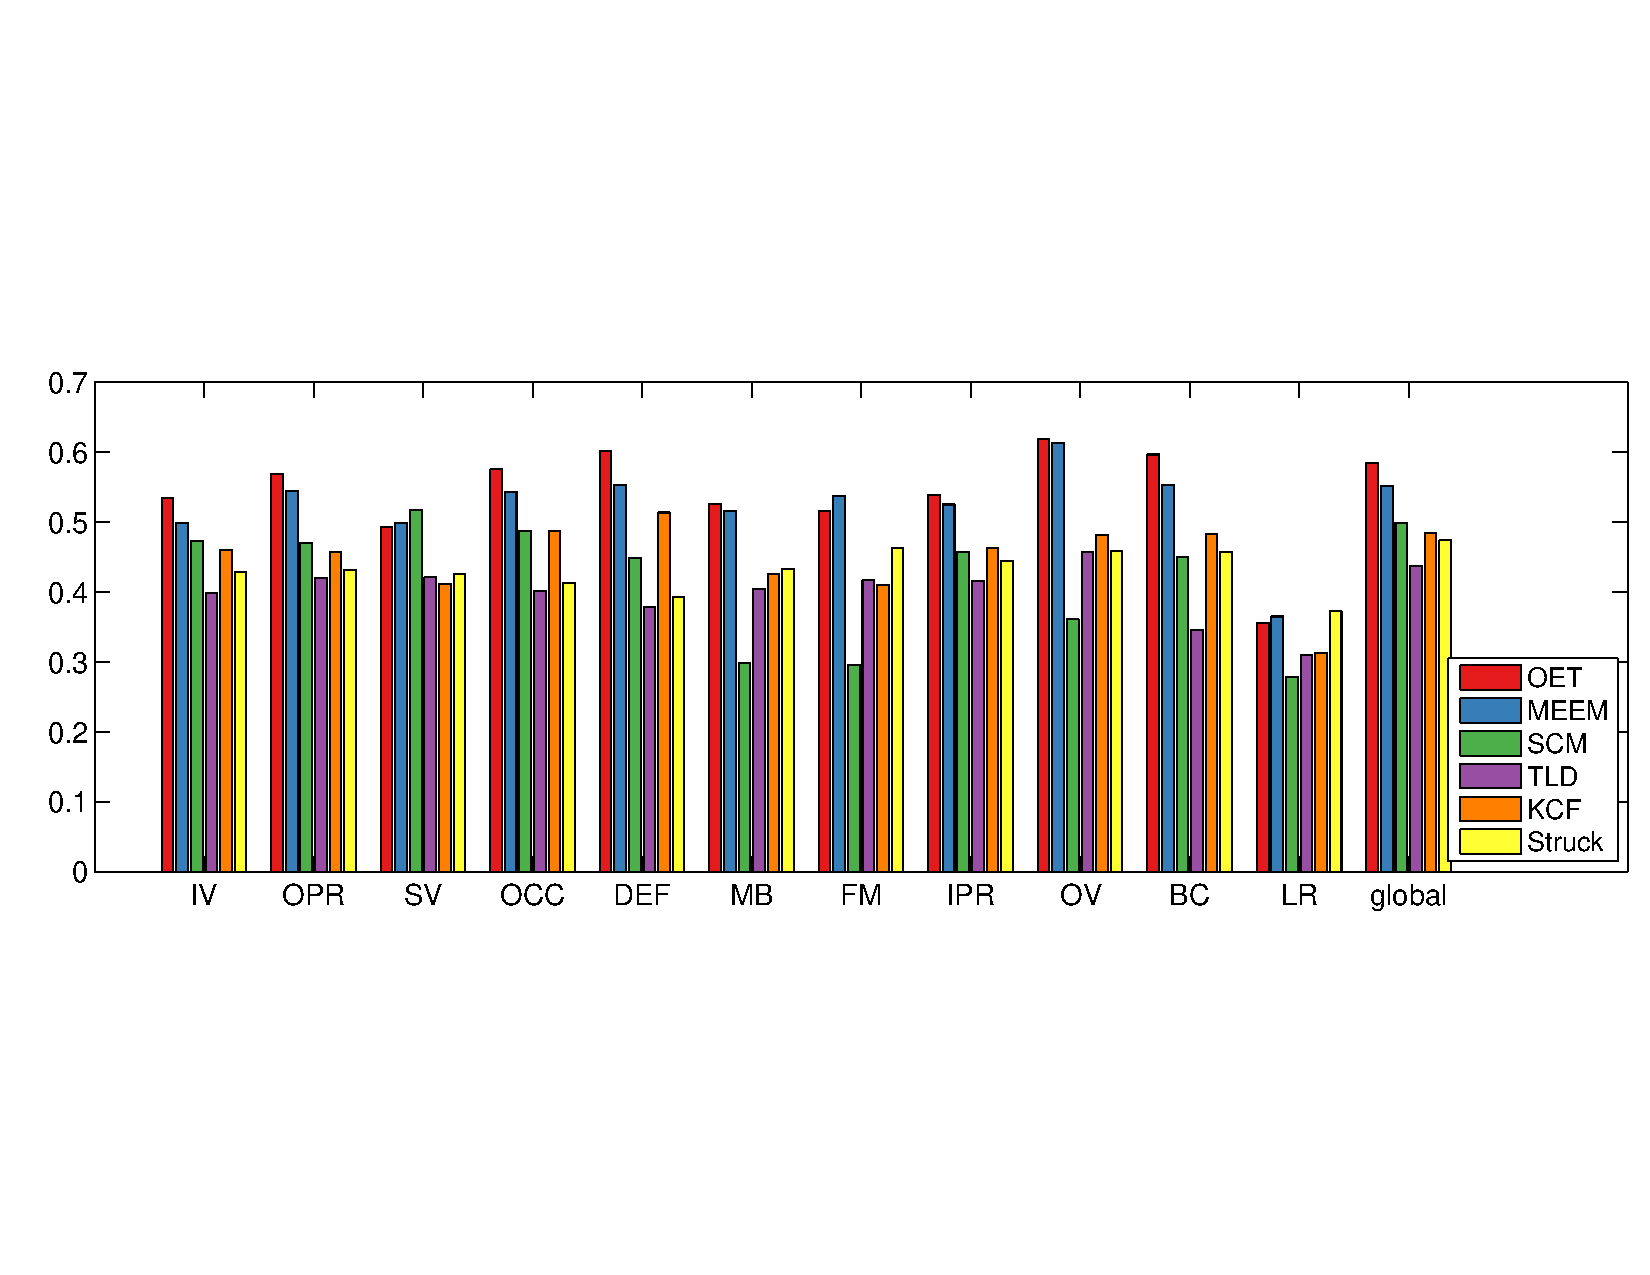
\includegraphics[width=1.0\linewidth, trim= 0.2cm 6.15cm 0.2cm 5.8cm, clip=true]{Figures/bar_graph.pdf}
\caption[Average AUC ranking scores of top trackers on different subsets of test
sequences in OPE]
{\small Average AUC ranking scores of top trackers on different subsets of test
		sequences in OPE. Each subset of sequences corresponds to an attribute:
		IV - illumination variation, OPR - out of plane rotation, SV- scale
		variation, OCC - occlusion, DEF - deformation, MB - motion blur, FM -
		fast motion, IPR - in plane rotation, OV - out of view, BC - background
		clutter, and LR - low resolution. Average AUC for all 50 videos is
		presented as global.}
\label{fig:attributes}
\end{figure}

The videos in the benchmark dataset are organized and selected with attributes,
which describe challenges present in the sequence - \eg occlusion, object
deformations. These properties are useful for diagnosing tracking behavior,
without the need of analyzing each video separately. Figure \ref{fig:attributes}
shows AUC ranking scores of recent trackers on different sequences, grouped by
attributes. For instance, background clutter (BC) contains all sequences whose
target pixels might be confused with background.

From figure \ref{fig:attributes}, our approach using appearance selection
outperforms other trackers in 8 of 11 attributes. Specifically, in attributes
such as IV (illumination variation), OPR (out of plane rotation), OCC
(occlusion), DEF (deformation), MB (motion blur), IPR (in plane rotation),
OV (out of view), and BC (background clutter). It is important to note that SCM
tracker is better than most recent trackers in terms of scale variation.
Results show that its affine motion models handle scale
variation better than other trackers, which are designed to account
translational motion \cite{Zhong2012}. In our system, scale is not determined. We
are dependent of each separated tracker scale, and some trackers do not consider
scale correction. Some of them apply initialization scale over all sequence.



